\documentclass[a4paper, 12pt]{article}
\usepackage{listings}
\usepackage{xcolor}
\usepackage{mathptmx}
\usepackage{graphicx}
\usepackage[T1]{fontenc}
\usepackage[section]{placeins}
\usepackage{fancyhdr}
\usepackage{lastpage}
\usepackage{enumitem}
\usepackage{amsfonts}
\usepackage{ulem}
\usepackage{blindtext}
\usepackage{hyperref}

\graphicspath{ {./images/} }

% Set left margin - The default is 1 inch, so the following
% command sets a 1.25-inch left margin.
\setlength{\oddsidemargin}{-0.25in}

% Set width of the text - What is left will be the right margin.
% In this case, right margin is 8.5in - 1.25in - 6in = 1.25in.
\setlength{\textwidth}{6.25in}

% Set top margin - The default is 1 inch, so the following
% command sets a 0.75-inch top margin.
\setlength{\topmargin}{-0.25in}

% Set height of the text - What is left will be the bottom margin.
% In this case, bottom margin is 11in - 0.75in - 9.5in = 0.75in
\setlength{\textheight}{8in}


\lstset{
    numberstyle=\tiny\color{gray},
    keywordstyle=\color{blue},
    commentstyle=\color{darkgray},
    stringstyle=\color{pink},
    tabsize=4,
    breaklines=true,
    breakatwhitespace=true,
    language=Oz
}

\pagestyle{fancy}
\headheight 29pt
\fancyhf{}
\rhead{Odd-Erik Frantzen}
\lhead{
    \raisebox{-0.33\height}{
\includegraphics[height=2em]{logo}}
    Final Report TDT4230
}
\rfoot{Page \thepage \hspace{1pt} of~\pageref{LastPage}}

\newenvironment{QandA}{\begin{enumerate}[label=\bfseries\alph*)]\bfseries}
{\end{enumerate}}
\newenvironment{answered}{\par\normalfont}{}

% Document
\title{Fur rendering with shells, fins, and order-independent transparency}
\date{2023\\ April}
\author{Odd-Erik Frantzen}
\begin{document}
    \maketitle
    \section{Introduction}
    I have chosen to work on fur rendering,
    using a variant of NVIDIA's shells and fins method.
    I've also implemented a form of order-independent transparency,
    as described in the paper Weighted Blended Order-Independent Transparency.
    I've also implemented a skybox, I use textures and object files, I use multiple shaders,
    and I use a custom framebuffer.
    You can move around the scene with WASD + Shift + Space,
    and you can turn the camera with the arrow keys.

    You can find my github repo here: \url{https://github.com/odderikf/fur_project}

    Make sure you run the binary from a subdirectory, like ./build or ./binaries.

    \section{Weighted Blended Order-Independent Transparency}

    Hair and fur notably have very fine detail, often sub-pixel,
    and therefore frequently need some form of blending to avoid jittery aliasing.
    Trying to depth sort hundreds or thousands of strands is of course, not trivial,
    so I've gone for a form of order-independent shading.

    Specifically, I've implemented a weighted order-independent 3-pass method,
    where the first pass is plainly rendered opaque geometry to the main framebuffer,
    the second pass does order-independent blending of semitransparent elements
    to its own framebuffer,
    and the third pass blends the transparent elements into the main framebuffer.
    A 4th pass can be done after this to add UI elements.

    This is based on the paper by Morgan McGuire and Louis Bavoil~\cite{McGuire2013Transparency}.
    An article on LearnOpenGL has been somewhat useful here~\cite{learnblended},
    as have the blog posts by one of the original authors of the paper~\cite{blendedblog1,blendedblog2,blendedblog3}.
    The LearnOpenGL article on framebuffers was very useful~\cite{learnframebuffers},
    as this method requires more complex framebuffer objects.

    The semitransparency pass has three channels:

    Accumulation stores the colored lit contribution to the blended product,
    based on their alpha, and their weight (a function of their distance in clip-space).
    It adds them to a separate accumulation buffer, with src=one, dst=one,
    so that the final result is the sum of all fragments.
    This means that blending happens through the in-shader weighting (alpha is multiplied into color for this).
    The alpha channel of accumulation stores their alpha times their weight,
    so that in the end, we can scale the accumulated color such that their alpha equals one.

    The revealage channel determines how much of the opaque scene
    to reveal through the semitransparent elements.
    This channel therefore clears to 1, fully revealing the opaque scene by default,
    and is then blended with src = 0, dst = 1-src,
    such that a visible fragment
    will lower the final revealage of the pass,
    hiding the opaque scene more.
    In the shader, the written value is simply the normal alpha of the object.

    Finally, the modulation output filters color out of the color channel from the opaque scene.
    This essentially lets color filters function as filters.
    This works by outputting (1 - color), adjusted for that fragments contribution (accumulation's alpha),
    the color being the fragment's material color, and not it's illuminated product.
    The blending mode is set to src=zero, dst= 1 - srccolor,
    so the modulation subtracts from the opaque scene's colors.

    The accumulated color is composited onto the color buffer,
    using the accumulation channel for color data,
    and the revealage channel to determine the alpha of this composite layer.

    Because OpenGL does not let you modify the default framebuffer,
    this solution creates its own framebuffer,
    and copies its final output into the default framebuffer at the end for display.

    \section{Fur rendering through Shells and Fins, using geometry shaders}

    Rendering individual fur strands requires an obscene amount of vertices,
    so shortcuts and cheats are naturally needed.
    One such cheat is the shell method,
    where you draw individual fur strands as dots on a 2d texture,
    on a shell around the model.
    By progressively stacking shells outwards,
    these dots form lines that can pass as strands of fur.

    The shell method works pretty great head-on,
    and you can imitate ambient shadows by just darkening the roots,
    but when viewing at an angle, you are able to see between the layers,
    which breaks the illusion.
    This can be alleviated by having fur cards, textured rectangles,
    that display fur strands.
    We can elect to generate these exclusively at the silhouette,
    to cover for the weak spot of the shell method.

    This method was described in a paper from 2001~\cite{Lengyel:2001:RFO}
    and a geometry-shader based approach was described by NVIDIA in 2007
    ~\cite{nvidiafur,nvidiasamples}

    I've mainly gone by intuition on these two techniques,
    other than that I've mainly looked at the NVIDIA paper.

    \subsection{Shells implementation}

    First, a fully opaque base is rendered,
    in the opaque pass.
    Then, we render the base again,
    but with a dedicated shader program.
    This shader program has a geometry shader,
    that takes in triangles,
    and generates several triangles displaced outwards.
    The local direction and length
    are determined by the color and alpha channels,
    respectively, of a texture,
    in addition to a uniform float for control of overall fur length.
    Using textures at a vertex level does of course,
    bottleneck the effective resolution of these textures by vertex density.
    This combing texture is in tangent space, so a TBN table must be used.

    The generated shells are then linearly spaced along this direction,
    and the usual preparations for lighting
    are calculated for each generated vertex.
    Additionally,
    thinning of hair is simulated by lowering alpha as you leave the scalp.
    So the normalized displacement as a third texture coordinate for 3d-textures.

    Additionally, as proof of concept,
    I've implemented a very basic wind displacement
    through uniform, that maintains length,
    but shifts fur directions somewhat along the wind.

    The fragment shader uses the blending method described above,
    uses phong lighting like most other elements in the scene,
    but slight rudimentary self-shadowing is implemented,
    by slightly darkening the roots and brightening the tips.
    Fur shells have their own normal map (blurred copy of the original,
    to soften perceived edges),
    and share their base's roughness map and color map.

    The final alpha of a pixel of shell is determined by
    its texture, a tip-thinning simulated by lowering alpha,
    and a turbulence/dots/fur density texture that determines which UV coordinates form strands.
    The python file gen\_fur\_density.py generates these dots textures.

    \subsection{Fins implementation}

    The fins are also implemented through a geometry shader.
    The NVIDIA paper suggests using adjacency input to find edges that form silhouettes,
    but I've opted to instead just use triangles input,
    and test every edge.
    This does lead to duplicates.

    For every triangle, it checks every edge.
    For each edge, if that edge's averaged vertex-normal
    is roughly perpendicular to the view direction,
    then generate a fur-card.
    A wide treshold is used, so that the cards can fade instead of pop in and out.
    These cards are also displaced along the fur direction, see the shells implementation,
    and can be generated with multiple vertices for deformation e.g.\ for wind or interaction.

    These silhouette fur-cards are rendered without back-face culling,
    as they cull themselves within reason,
    and this saves worrying about winding order and facing
    The fragment shader shares most of its details with the shells shader,
    though notably the fins do not use normal maps, roughness maps, or a dots texture.

    \section{Skybox}
    A basic skybox is set up.
    It is drawn as the first opaque element,
    has a box mesh,
    uses position for UVs,
    isn't lit,
    and has gl\_Position set to xyww,
    so that it is always at the maximum distance in clipspace.
    Depth testing uses less-than-equal because of this.
    I've used a free skybox texture named Yokohama2~\cite{yokohama2}.
    The tutorial of cubemaps and skyboxes from LearnOpenGL was useful here~\cite{learncubemaps}

    \section{Workflow, filetypes, libraries}
    The blender directory in the github repo (not included in code zip) contains a couple of blender projects.
    They have various setup done.
    Ricky.blend contains the mouse,
    and has shaders set up to emulate some of the rendering techniques,
    for more representative texture painting.
    Ricky features a normal map baked from a displacement map, which was done in blender.

    fur\_project.blend contains the grass-covered terrain, the broad terrain,
    and an export script in python.

    For object loading, I've used tinyobjloader.
    For PNG loading, I've used the given utility file, which uses lodepng.
    For OpenGL support, I've used GLAD, the python GLAD generator, GLFW window loader, and GLM maths library.
    For string processing, I've used fmt, a text formatting library.
    All of these libraries are included as git submodules, and are linked, included, and compiled through my CMakeLists file.

    \section{Troubles and tribulations}
    It took me a while to figure out a good weighting for the blending operator,
    as the paper is somewhat cryptic,
    and no other resources I found made things much clearer.
    I ended up picking formula 10, which uses fragment coordinates,
    and tweaking the results until the fur behaved.
    You can tell that the pads become less transparent as you get far away from them,
    I imagine there's more tweaking I can do to perfect these weights,
    but these weights and the difficulty/impossibility of perfecting them for arbitrary scenes
    are also a flaw of this method.

    I decided to implement the color modulation/transmission blending variant described in the third blog post eventually,
    thinking it would solve a problem I had with blending,
    when really the main problem there was the weight function.
    I've still gotten it roughly working, I think, but it ended up being mostly unnecessary work.

    I ultimately wished to make a new animal model,
    as ricky the rat is neither pretty nor well mapped,
    but decided to focus on technical things instead.
    Might make something for the presentation though.

    For ages, the way I generated tangents was flawed,
    and it took me an embarassing amount of time to even fully realize.
    Ultimately the problem seems to have been a lack of normalization.

    \newpage
    \section*{Appendix}

    \subsection*{Cool JPGs}

    Here's the full scene.
    You can see intersecting,
    overlapping, textured, normal-mapped, roughness mapped semitransparent paddles on the right,
    showing off the blending.
    Below the paddles is a grass/fur covered field.
    Behind the field and hill is a skybox,
    rendered on top of all this is a text overlay,
    and to the left is the fur-covered rat.
    The scene has three colored lights
    (alas, no visual representation of their sources),
    as well as a fourth high in the sky with very high intensity,
    to act like the sun.
    The sun should probably be a dirlight instead of a pointlight,
    but I ended up never making the time for the implementation.


    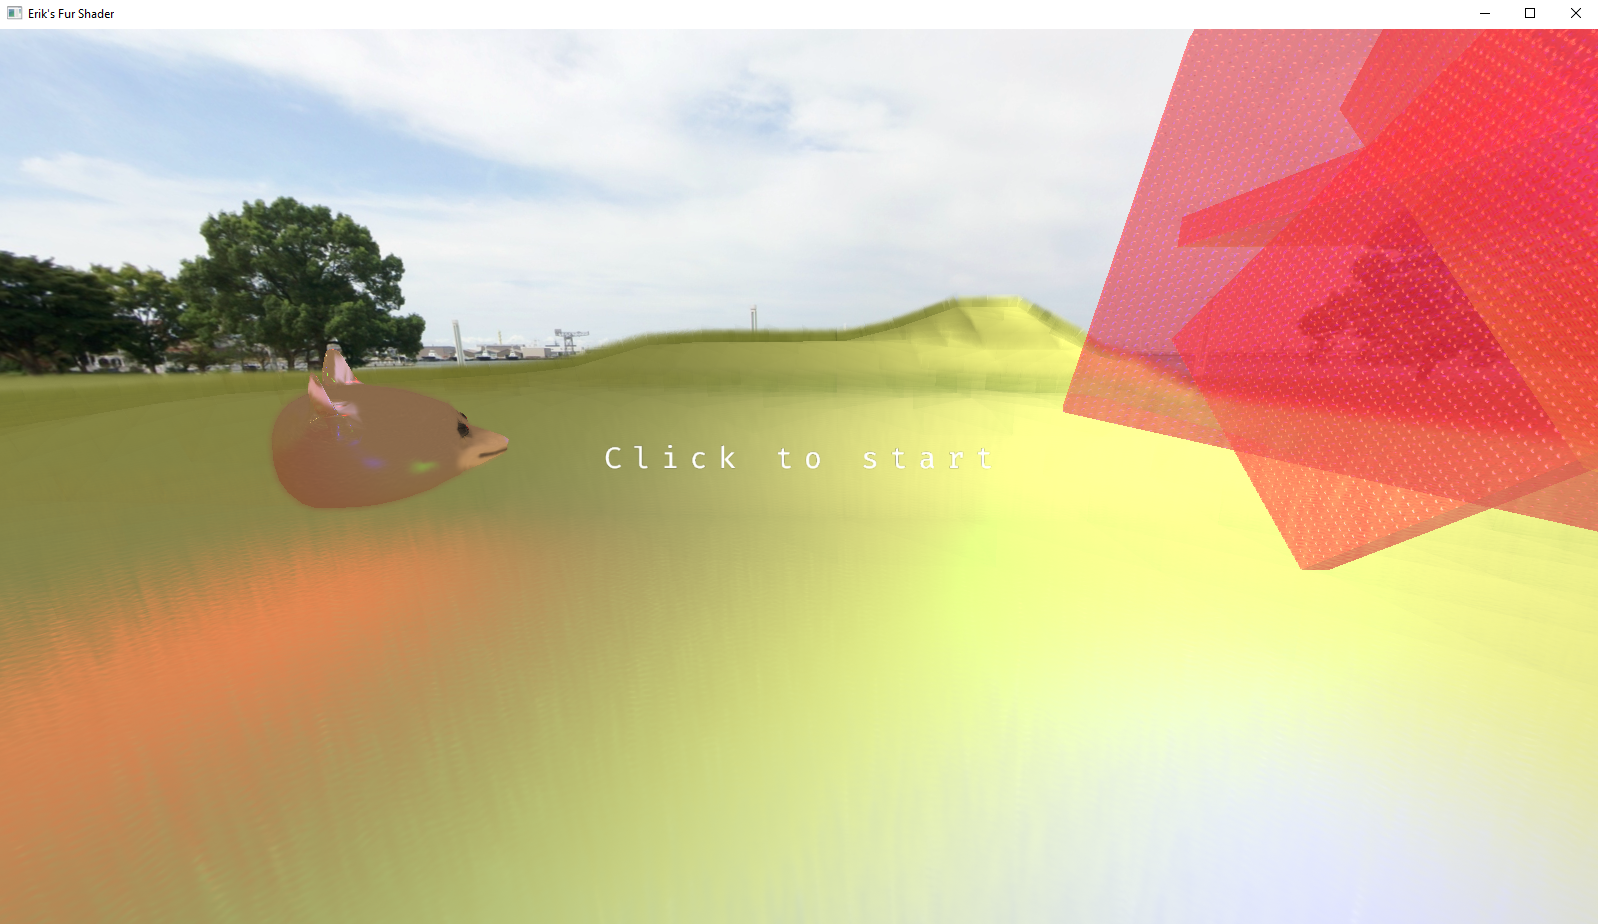
\includegraphics[width=35em]{fullscene}

    Here's a closeup of the overlapping pads.
    You can definitely see some blending artifacts with the grass here,
    but tuning the weights to never have any of that happen is difficult.

    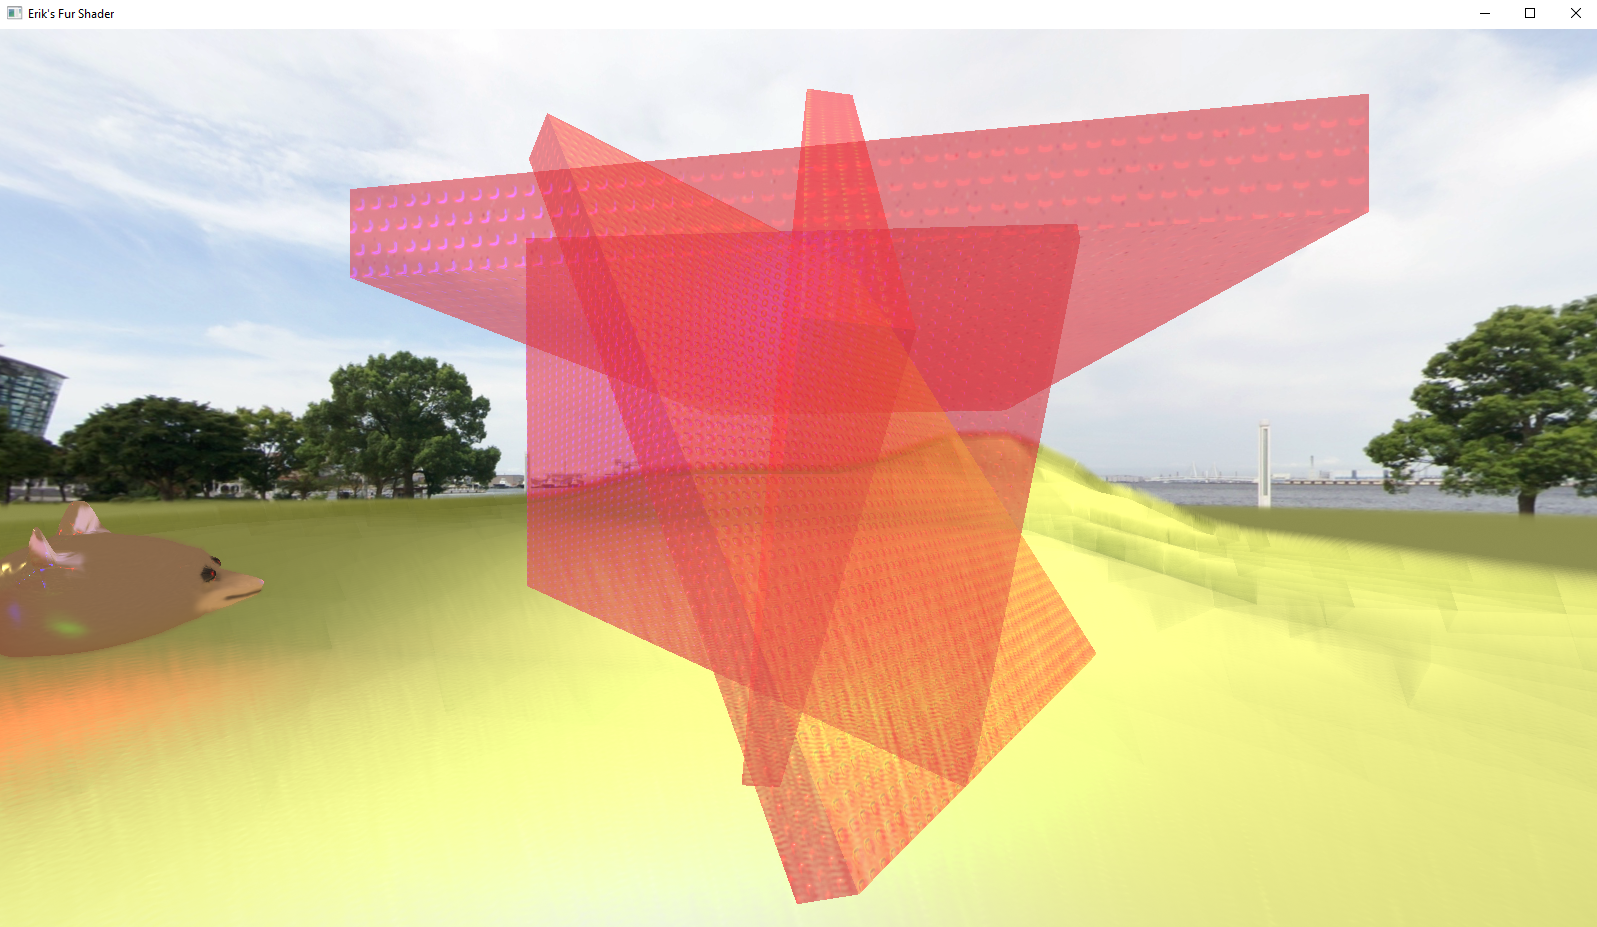
\includegraphics[width=35em]{overlap}

    Here's a view of below the grass shells,
    so you pretty much just see the fins.
    The ground has very big polygons, so the fins struggle to actually cover them well.
    There could definitely be some more graceful fading in and out of fins vs shells here.

    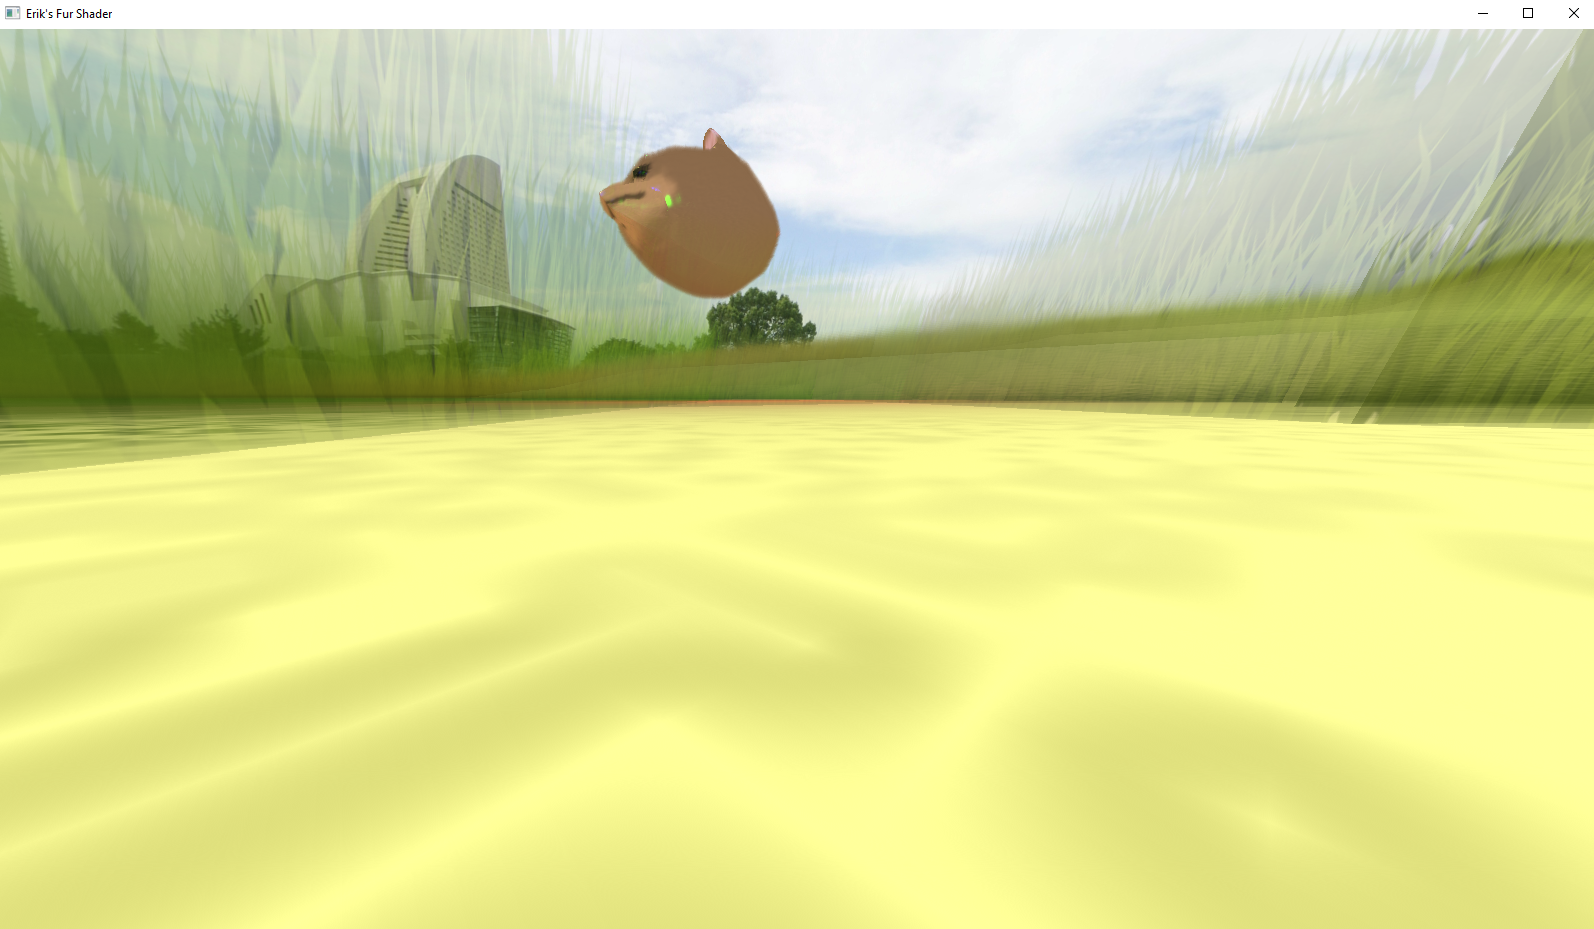
\includegraphics[width=35em]{grounded}


    Here's a closeup of the rat,
    you can see that the fur is fairly groomed,
    and parts like the eyes and the nose have no fur on them, since the alpha of the fur texture is zero there.

    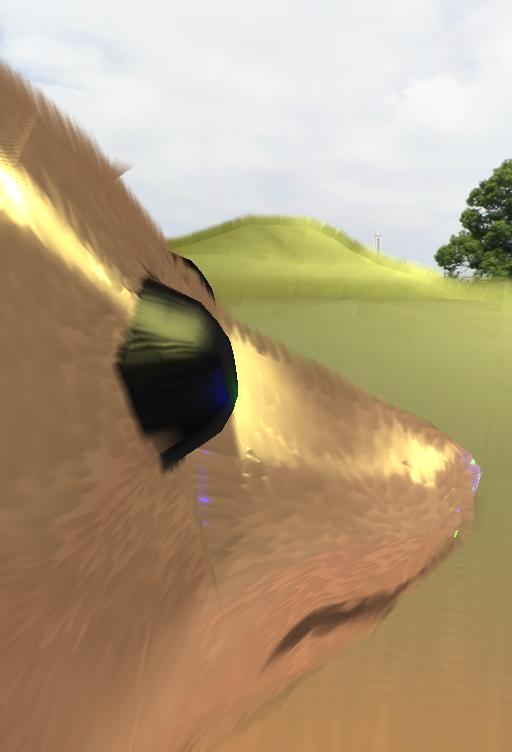
\includegraphics[width=35em]{groomed}

    As you can see here, blended things are still occluded by the opaque bases.

    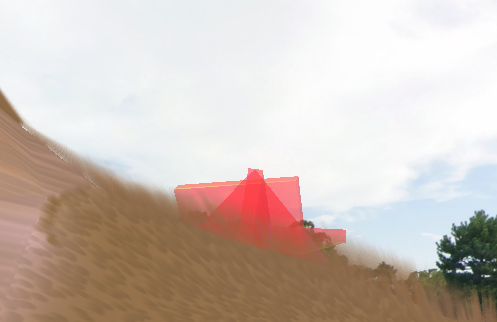
\includegraphics[width=35em]{depth}

    Here's the scene without shells

    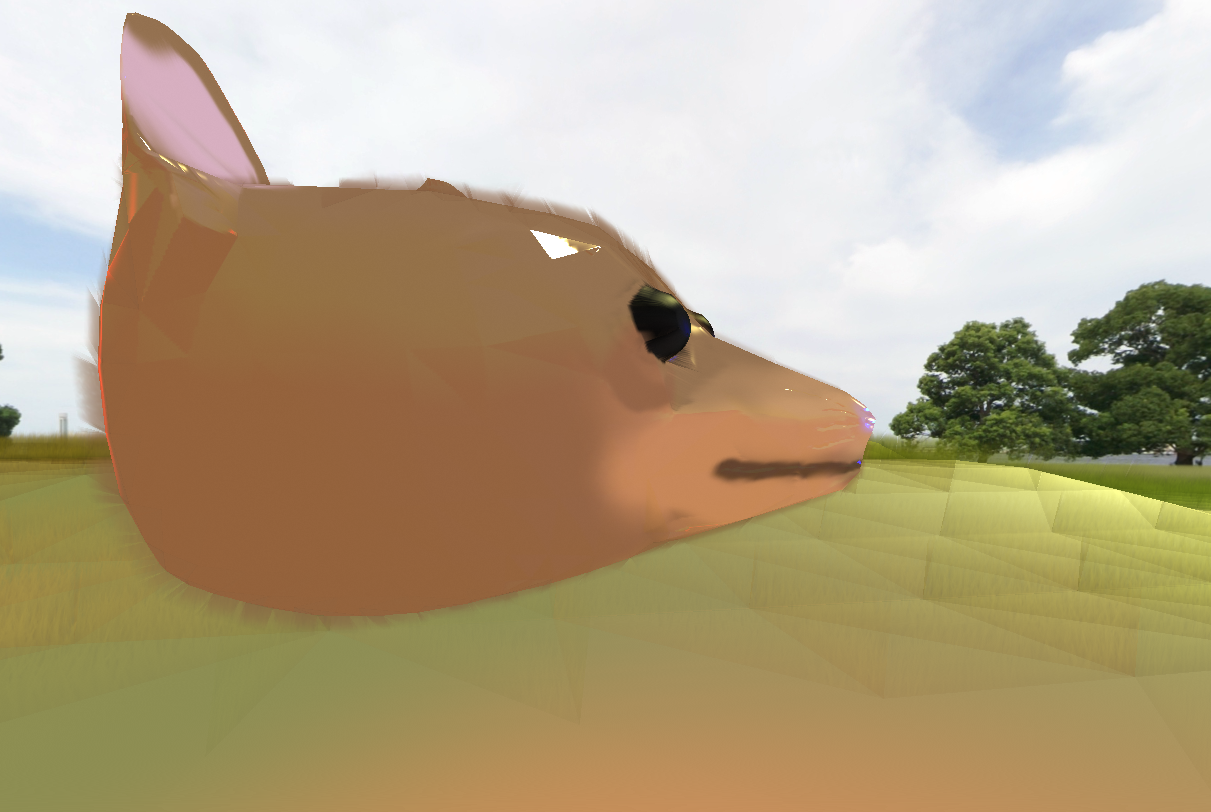
\includegraphics[width=35em]{fins}

    Here's the scene without fins

    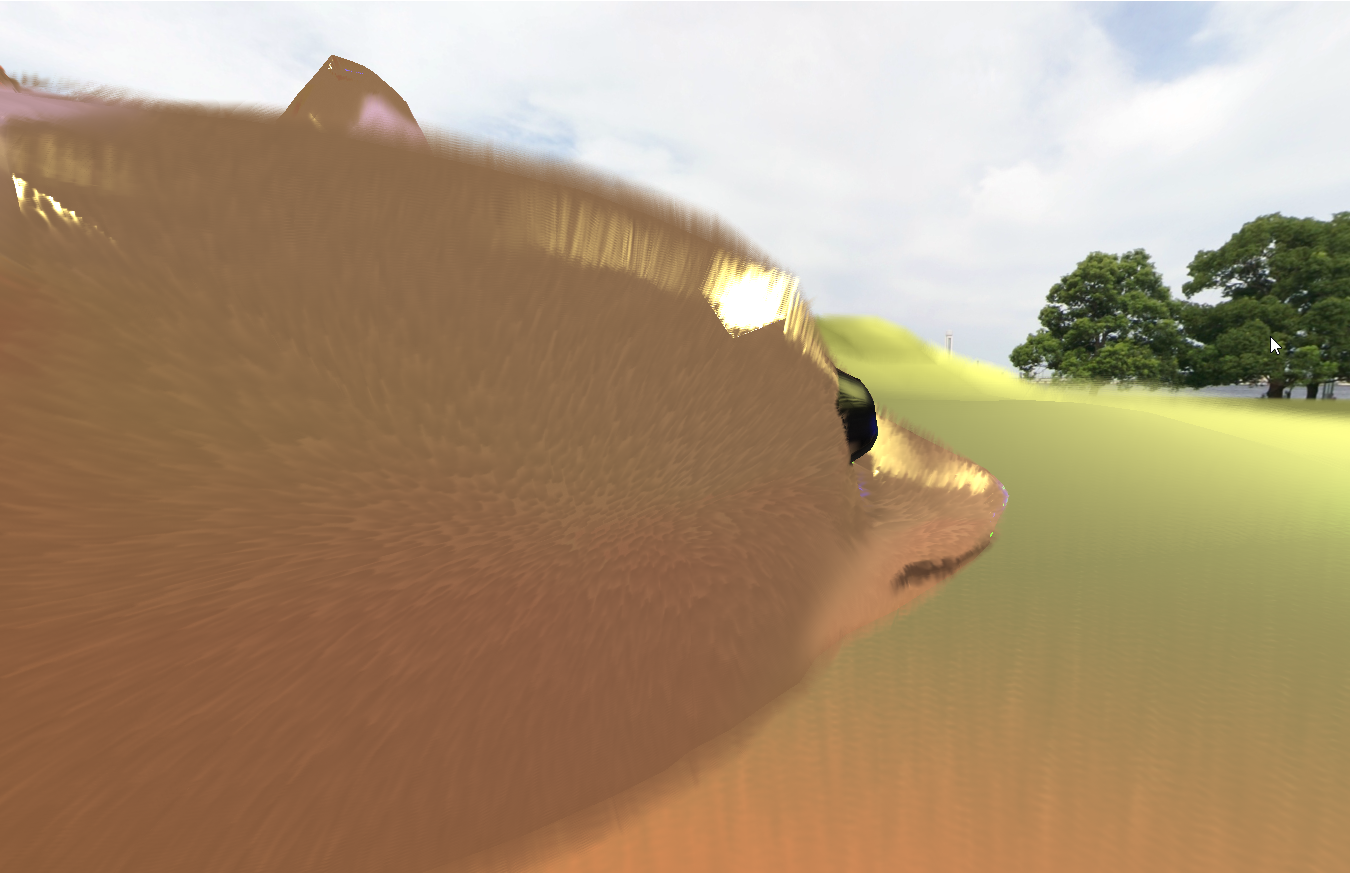
\includegraphics[width=35em]{shells}

    Here's the scene with both enabled again

    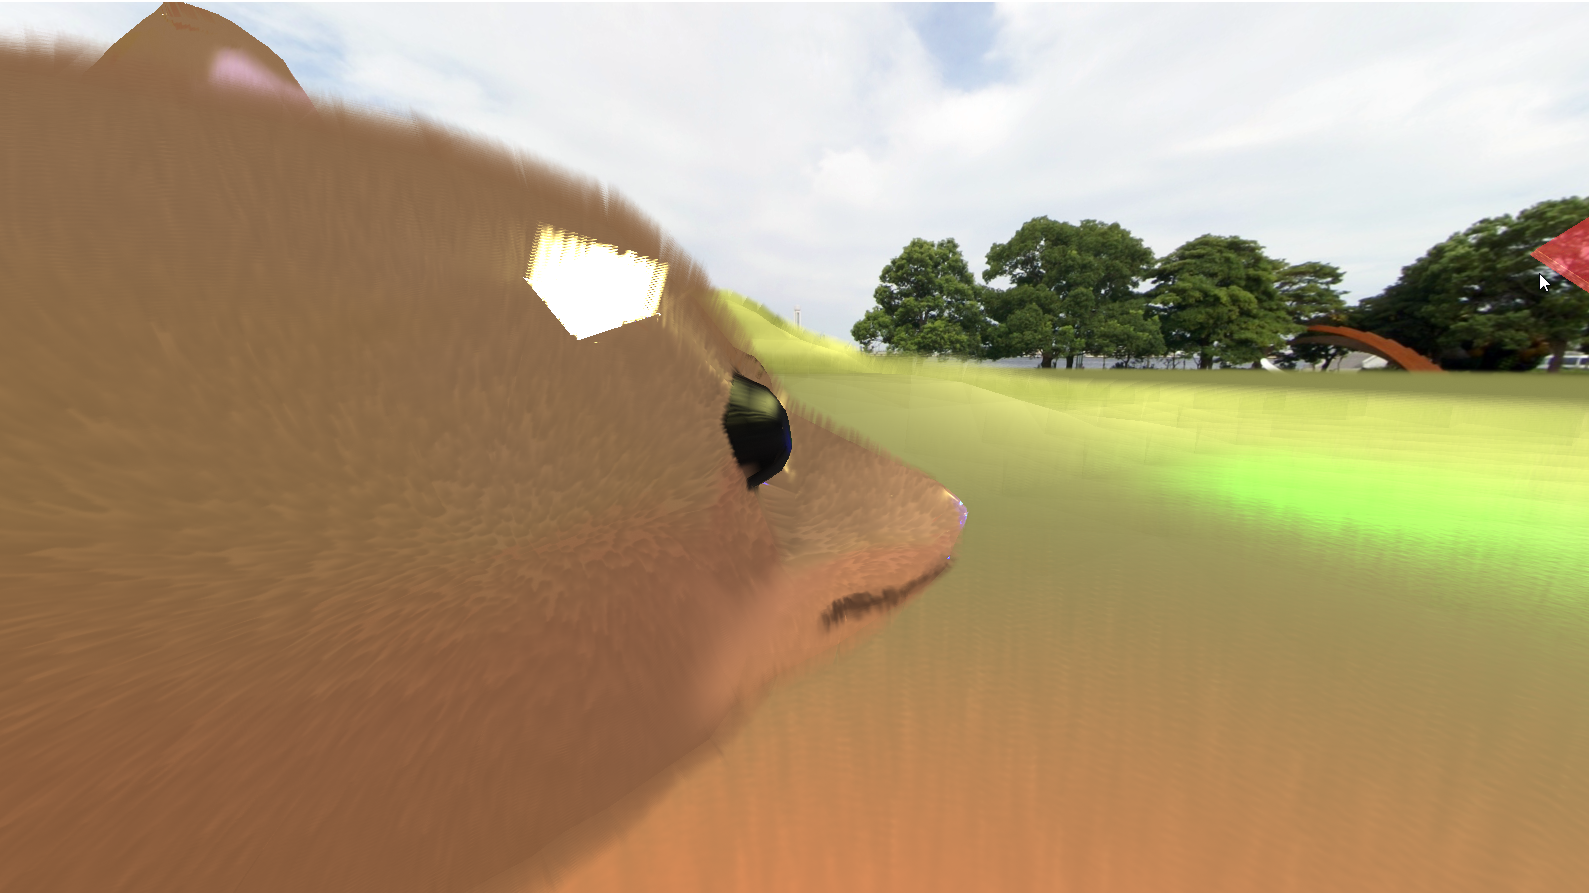
\includegraphics[width=35em]{both}





    \bibliography{refs}
    \bibliographystyle{ieeetr}

\end{document}